\documentclass[1p]{elsarticle_modified}
%\bibliographystyle{elsarticle-num}

%\usepackage[colorlinks]{hyperref}
%\usepackage{abbrmath_seonhwa} %\Abb, \Ascr, \Acal ,\Abf, \Afrak
\usepackage{amsfonts}
\usepackage{amssymb}
\usepackage{amsmath}
\usepackage{amsthm}
\usepackage{scalefnt}
\usepackage{amsbsy}
\usepackage{kotex}
\usepackage{caption}
\usepackage{subfig}
\usepackage{color}
\usepackage{graphicx}
\usepackage{xcolor} %% white, black, red, green, blue, cyan, magenta, yellow
\usepackage{float}
\usepackage{setspace}
\usepackage{hyperref}

\usepackage{tikz}
\usetikzlibrary{arrows}

\usepackage{multirow}
\usepackage{array} % fixed length table
\usepackage{hhline}

%%%%%%%%%%%%%%%%%%%%%
\makeatletter
\renewcommand*\env@matrix[1][\arraystretch]{%
	\edef\arraystretch{#1}%
	\hskip -\arraycolsep
	\let\@ifnextchar\new@ifnextchar
	\array{*\c@MaxMatrixCols c}}
\makeatother %https://tex.stackexchange.com/questions/14071/how-can-i-increase-the-line-spacing-in-a-matrix
%%%%%%%%%%%%%%%

\usepackage[normalem]{ulem}

\newcommand{\msout}[1]{\ifmmode\text{\sout{\ensuremath{#1}}}\else\sout{#1}\fi}
%SOURCE: \msout is \stkout macro in https://tex.stackexchange.com/questions/20609/strikeout-in-math-mode

\newcommand{\cancel}[1]{
	\ifmmode
	{\color{red}\msout{#1}}
	\else
	{\color{red}\sout{#1}}
	\fi
}

\newcommand{\add}[1]{
	{\color{blue}\uwave{#1}}
}

\newcommand{\replace}[2]{
	\ifmmode
	{\color{red}\msout{#1}}{\color{blue}\uwave{#2}}
	\else
	{\color{red}\sout{#1}}{\color{blue}\uwave{#2}}
	\fi
}

\newcommand{\Sol}{\mathcal{S}} %segment
\newcommand{\D}{D} %diagram
\newcommand{\A}{\mathcal{A}} %arc


%%%%%%%%%%%%%%%%%%%%%%%%%%%%%5 test

\def\sl{\operatorname{\textup{SL}}(2,\Cbb)}
\def\psl{\operatorname{\textup{PSL}}(2,\Cbb)}
\def\quan{\mkern 1mu \triangleright \mkern 1mu}

\theoremstyle{definition}
\newtheorem{thm}{Theorem}[section]
\newtheorem{prop}[thm]{Proposition}
\newtheorem{lem}[thm]{Lemma}
\newtheorem{ques}[thm]{Question}
\newtheorem{cor}[thm]{Corollary}
\newtheorem{defn}[thm]{Definition}
\newtheorem{exam}[thm]{Example}
\newtheorem{rmk}[thm]{Remark}
\newtheorem{alg}[thm]{Algorithm}

\newcommand{\I}{\sqrt{-1}}
\begin{document}

%\begin{frontmatter}
%
%\title{Boundary parabolic representations of knots up to 8 crossings}
%
%%% Group authors per affiliation:
%\author{Yunhi Cho} 
%\address{Department of Mathematics, University of Seoul, Seoul, Korea}
%\ead{yhcho@uos.ac.kr}
%
%
%\author{Seonhwa Kim} %\fnref{s_kim}}
%\address{Center for Geometry and Physics, Institute for Basic Science, Pohang, 37673, Korea}
%\ead{ryeona17@ibs.re.kr}
%
%\author{Hyuk Kim}
%\address{Department of Mathematical Sciences, Seoul National University, Seoul 08826, Korea}
%\ead{hyukkim@snu.ac.kr}
%
%\author{Seokbeom Yoon}
%\address{Department of Mathematical Sciences, Seoul National University, Seoul, 08826,  Korea}
%\ead{sbyoon15@snu.ac.kr}
%
%\begin{abstract}
%We find all boundary parabolic representation of knots up to 8 crossings.
%
%\end{abstract}
%\begin{keyword}
%    \MSC[2010] 57M25 
%\end{keyword}
%
%\end{frontmatter}

%\linenumbers
%\tableofcontents
%
\newcommand\colored[1]{\textcolor{white}{\rule[-0.35ex]{0.8em}{1.4ex}}\kern-0.8em\color{red} #1}%
%\newcommand\colored[1]{\textcolor{white}{ #1}\kern-2.17ex	\textcolor{white}{ #1}\kern-1.81ex	\textcolor{white}{ #1}\kern-2.15ex\color{red}#1	}

{\Large $\underline{12n_{0100}~(K12n_{0100})}$}

\setlength{\tabcolsep}{10pt}
\renewcommand{\arraystretch}{1.6}
\vspace{1cm}\begin{tabular}{m{100pt}>{\centering\arraybackslash}m{274pt}}
\multirow{5}{120pt}{
	\centering
	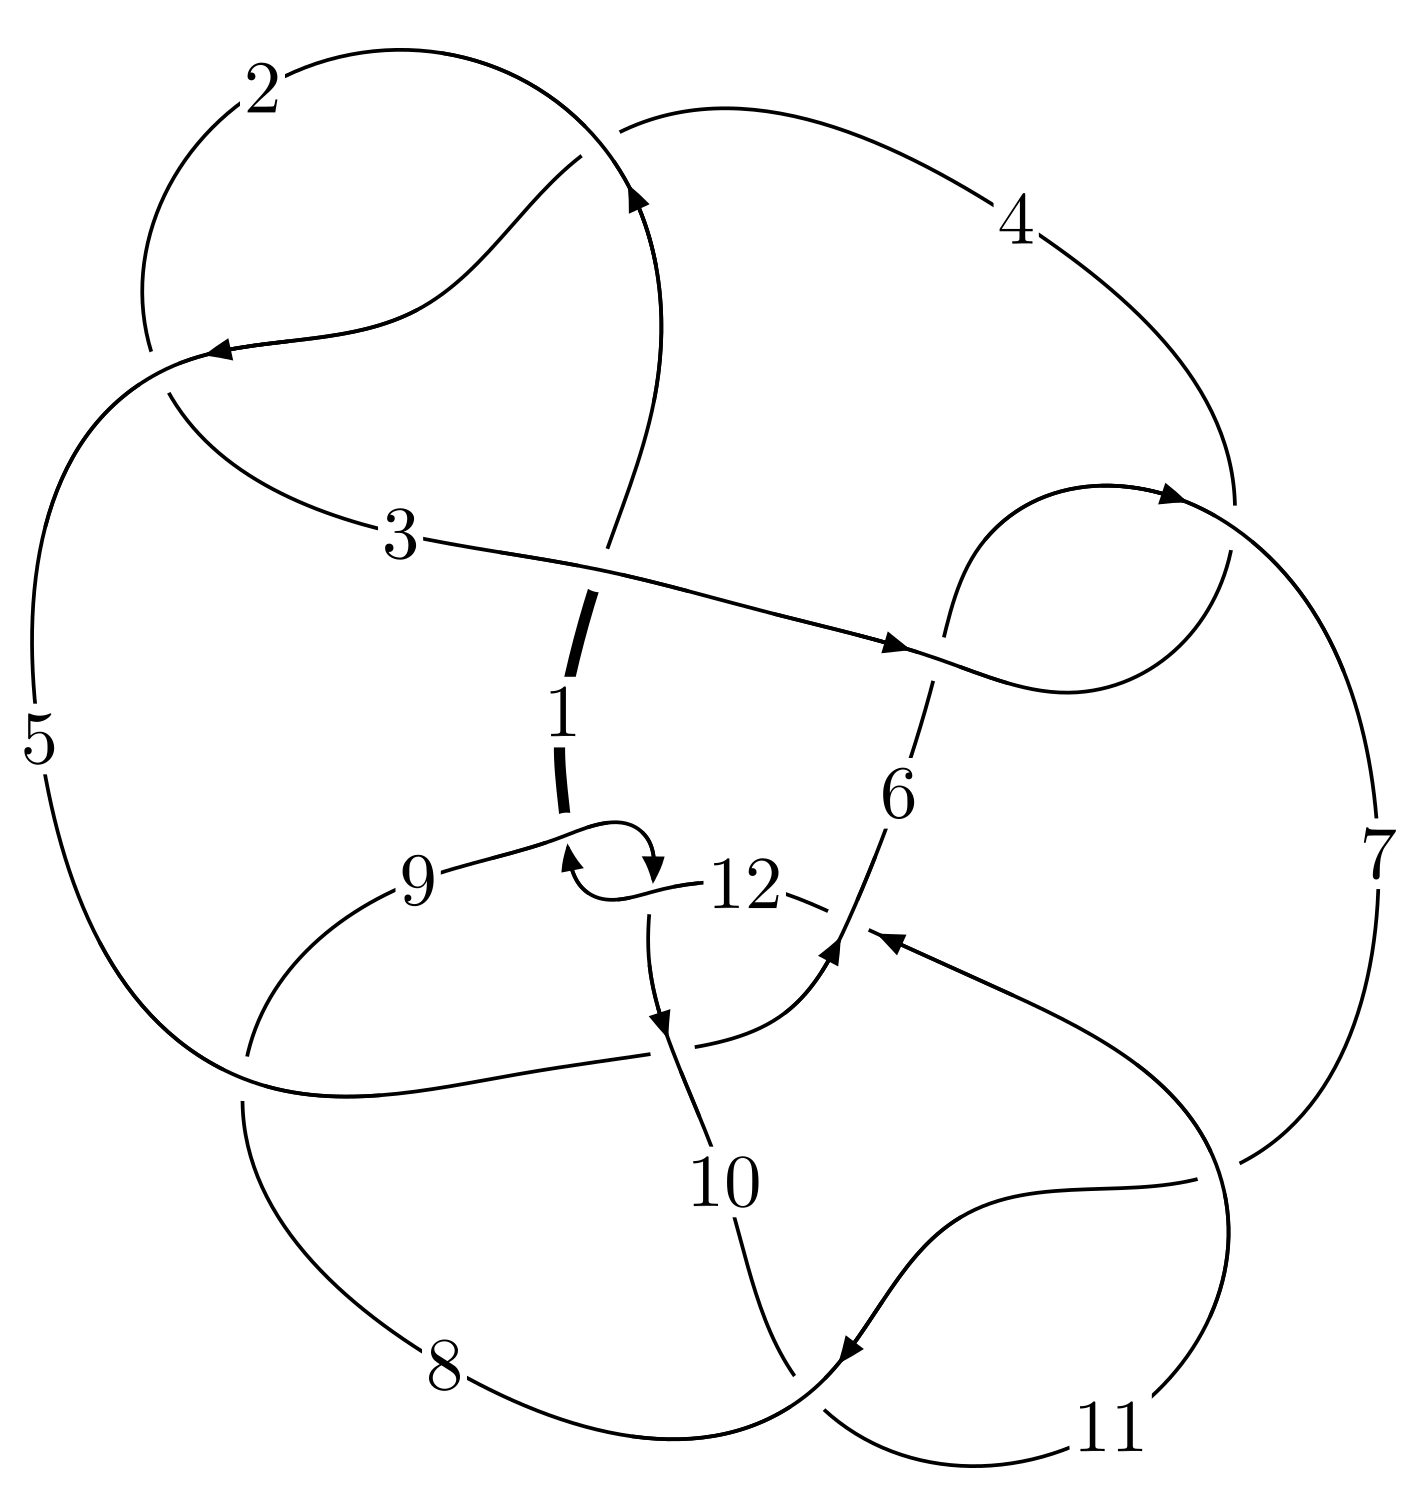
\includegraphics[width=112pt]{../../../GIT/diagram.site/Diagrams/png/2189_12n_0100.png}\\
\ \ \ A knot diagram\footnotemark}&
\allowdisplaybreaks
\textbf{Linearized knot diagam} \\
\cline{2-2}
 &
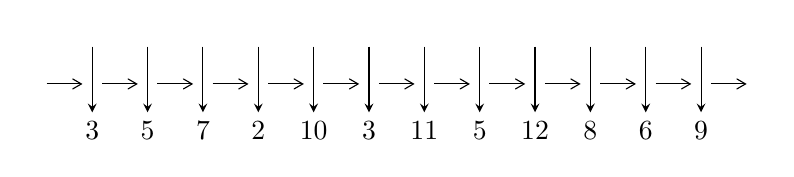
\begin{tikzpicture}[x=20pt, y=17pt]
	% nodes
	\node (C0) at (0, 0) {};
	\node (C1) at (1, 0) {};
	\node (C1U) at (1, +1) {};
	\node (C1D) at (1, -1) {3};

	\node (C2) at (2, 0) {};
	\node (C2U) at (2, +1) {};
	\node (C2D) at (2, -1) {5};

	\node (C3) at (3, 0) {};
	\node (C3U) at (3, +1) {};
	\node (C3D) at (3, -1) {7};

	\node (C4) at (4, 0) {};
	\node (C4U) at (4, +1) {};
	\node (C4D) at (4, -1) {2};

	\node (C5) at (5, 0) {};
	\node (C5U) at (5, +1) {};
	\node (C5D) at (5, -1) {10};

	\node (C6) at (6, 0) {};
	\node (C6U) at (6, +1) {};
	\node (C6D) at (6, -1) {3};

	\node (C7) at (7, 0) {};
	\node (C7U) at (7, +1) {};
	\node (C7D) at (7, -1) {11};

	\node (C8) at (8, 0) {};
	\node (C8U) at (8, +1) {};
	\node (C8D) at (8, -1) {5};

	\node (C9) at (9, 0) {};
	\node (C9U) at (9, +1) {};
	\node (C9D) at (9, -1) {12};

	\node (C10) at (10, 0) {};
	\node (C10U) at (10, +1) {};
	\node (C10D) at (10, -1) {8};

	\node (C11) at (11, 0) {};
	\node (C11U) at (11, +1) {};
	\node (C11D) at (11, -1) {6};

	\node (C12) at (12, 0) {};
	\node (C12U) at (12, +1) {};
	\node (C12D) at (12, -1) {9};
	\node (C13) at (13, 0) {};

	% arrows
	\draw[->,>={angle 60}]
	(C0) edge (C1) (C1) edge (C2) (C2) edge (C3) (C3) edge (C4) (C4) edge (C5) (C5) edge (C6) (C6) edge (C7) (C7) edge (C8) (C8) edge (C9) (C9) edge (C10) (C10) edge (C11) (C11) edge (C12) (C12) edge (C13) ;	\draw[->,>=stealth]
	(C1U) edge (C1D) (C2U) edge (C2D) (C3U) edge (C3D) (C4U) edge (C4D) (C5U) edge (C5D) (C6U) edge (C6D) (C7U) edge (C7D) (C8U) edge (C8D) (C9U) edge (C9D) (C10U) edge (C10D) (C11U) edge (C11D) (C12U) edge (C12D) ;
	\end{tikzpicture} \\
\hhline{~~} \\& 
\textbf{Solving Sequence} \\ \cline{2-2} 
 &
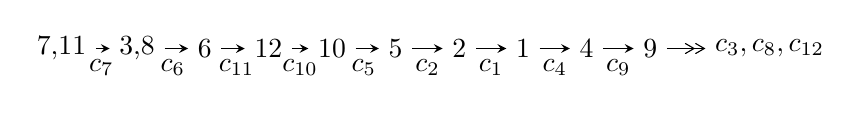
\begin{tikzpicture}[x=23pt, y=7pt]
	% node
	\node (A0) at (-1/8, 0) {7,11};
	\node (A1) at (17/16, 0) {3,8};
	\node (A2) at (17/8, 0) {6};
	\node (A3) at (25/8, 0) {12};
	\node (A4) at (33/8, 0) {10};
	\node (A5) at (41/8, 0) {5};
	\node (A6) at (49/8, 0) {2};
	\node (A7) at (57/8, 0) {1};
	\node (A8) at (65/8, 0) {4};
	\node (A9) at (73/8, 0) {9};
	\node (C1) at (1/2, -1) {$c_{7}$};
	\node (C2) at (13/8, -1) {$c_{6}$};
	\node (C3) at (21/8, -1) {$c_{11}$};
	\node (C4) at (29/8, -1) {$c_{10}$};
	\node (C5) at (37/8, -1) {$c_{5}$};
	\node (C6) at (45/8, -1) {$c_{2}$};
	\node (C7) at (53/8, -1) {$c_{1}$};
	\node (C8) at (61/8, -1) {$c_{4}$};
	\node (C9) at (69/8, -1) {$c_{9}$};
	\node (A10) at (11, 0) {$c_{3},c_{8},c_{12}$};

	% edge
	\draw[->,>=stealth]	
	(A0) edge (A1) (A1) edge (A2) (A2) edge (A3) (A3) edge (A4) (A4) edge (A5) (A5) edge (A6) (A6) edge (A7) (A7) edge (A8) (A8) edge (A9) ;
	\draw[->>,>={angle 60}]	
	(A9) edge (A10);
\end{tikzpicture} \\ 

\end{tabular} \\

\footnotetext{
The image of knot diagram is generated by the software ``\textbf{Draw programme}" developed by Andrew Bartholomew(\url{http://www.layer8.co.uk/maths/draw/index.htm\#Running-draw}), where we modified some parts for our purpose(\url{https://github.com/CATsTAILs/LinksPainter}).
}\phantom \\ \newline 
\centering \textbf{Ideals for irreducible components\footnotemark of $X_{\text{par}}$} 
 
\begin{align*}
I^u_{1}&=\langle 
10938104279 u^{29}+17799069811 u^{28}+\cdots+790454724608 b+452983966639,\\
\phantom{I^u_{1}}&\phantom{= \langle  }3054129323185 u^{29}-6949903407647 u^{28}+\cdots+6323637796864 a-16733471682507,\\
\phantom{I^u_{1}}&\phantom{= \langle  }u^{30}-2 u^{29}+\cdots-6 u+1\rangle \\
I^u_{2}&=\langle 
-1.61369\times10^{45} u^{39}-9.40408\times10^{45} u^{38}+\cdots+2.40030\times10^{46} b-2.57635\times10^{47},\\
\phantom{I^u_{2}}&\phantom{= \langle  }-2.95178\times10^{47} u^{39}-1.77493\times10^{48} u^{38}+\cdots+2.32829\times10^{48} a-4.68541\times10^{49},\\
\phantom{I^u_{2}}&\phantom{= \langle  }u^{40}+6 u^{39}+\cdots+666 u+97\rangle \\
I^u_{3}&=\langle 
b,\;5 u^2+4 a+3 u+11,\;u^3+2 u-1\rangle \\
I^u_{4}&=\langle 
-12 a^2 u+91 a^2-564 a u+337 b+570 a+188 u+147,\;a^3-5 a^2 u+7 a^2+4 a u+a+2 u+1,\;u^2+1\rangle \\
I^u_{5}&=\langle 
b,\;u^3+a+u,\;u^4+u^3+2 u^2+2 u+1\rangle \\
I^u_{6}&=\langle 
3 b-2 a-2,\;4 a^2+2 a-11,\;u-1\rangle \\
\\
\end{align*}
\raggedright * 6 irreducible components of $\dim_{\mathbb{C}}=0$, with total 85 representations.\\
\footnotetext{All coefficients of polynomials are rational numbers. But the coefficients are sometimes approximated in decimal forms when there is not enough margin.}
\newpage
\renewcommand{\arraystretch}{1}
\centering \section*{I. $I^u_{1}= \langle 1.09\times10^{10} u^{29}+1.78\times10^{10} u^{28}+\cdots+7.90\times10^{11} b+4.53\times10^{11},\;3.05\times10^{12} u^{29}-6.95\times10^{12} u^{28}+\cdots+6.32\times10^{12} a-1.67\times10^{13},\;u^{30}-2 u^{29}+\cdots-6 u+1 \rangle$}
\flushleft \textbf{(i) Arc colorings}\\
\begin{tabular}{m{7pt} m{180pt} m{7pt} m{180pt} }
\flushright $a_{7}=$&$\begin{pmatrix}1\\0\end{pmatrix}$ \\
\flushright $a_{11}=$&$\begin{pmatrix}0\\u\end{pmatrix}$ \\
\flushright $a_{3}=$&$\begin{pmatrix}-0.482970 u^{29}+1.09904 u^{28}+\cdots-14.1778 u+2.64618\\-0.0138377 u^{29}-0.0225175 u^{28}+\cdots-0.0339714 u-0.573068\end{pmatrix}$ \\
\flushright $a_{8}=$&$\begin{pmatrix}1\\u^2\end{pmatrix}$ \\
\flushright $a_{6}=$&$\begin{pmatrix}-0.269448 u^{29}+0.688032 u^{28}+\cdots-10.5362 u+2.79507\\-0.306258 u^{29}+0.647053 u^{28}+\cdots+0.353711 u-0.471726\end{pmatrix}$ \\
\flushright $a_{12}=$&$\begin{pmatrix}0.000122070 u^{29}-0.000366211 u^{28}+\cdots+1.99915 u-0.999878\\0.000244141 u^{29}-0.000732422 u^{28}+\cdots+1.99829 u+0.000244141\end{pmatrix}$ \\
\flushright $a_{10}=$&$\begin{pmatrix}u\\u^3+u\end{pmatrix}$ \\
\flushright $a_{5}=$&$\begin{pmatrix}-0.198114 u^{29}+0.535158 u^{28}+\cdots-10.9040 u+2.84822\\-0.159014 u^{29}+0.310603 u^{28}+\cdots-0.146693 u-0.408378\end{pmatrix}$ \\
\flushright $a_{2}=$&$\begin{pmatrix}-0.116259 u^{29}+0.299479 u^{28}+\cdots-6.99440 u+1.41903\\-0.159014 u^{29}+0.310603 u^{28}+\cdots-0.146693 u-0.408378\end{pmatrix}$ \\
\flushright $a_{1}=$&$\begin{pmatrix}-0.000244141 u^{29}+0.000732422 u^{28}+\cdots-1.99829 u+0.999756\\-0.000488281 u^{29}+0.00146484 u^{28}+\cdots-1.99658 u-0.000488281\end{pmatrix}$ \\
\flushright $a_{4}=$&$\begin{pmatrix}-0.469133 u^{29}+1.12155 u^{28}+\cdots-14.1438 u+3.21925\\-0.0138377 u^{29}-0.0225175 u^{28}+\cdots-0.0339714 u-0.573068\end{pmatrix}$ \\
\flushright $a_{9}=$&$\begin{pmatrix}0.000122070 u^{29}-0.000366211 u^{28}+\cdots+1.99915 u+0.000122070\\0.000244141 u^{29}-0.000732422 u^{28}+\cdots+0.998291 u+0.000244141\end{pmatrix}$\\&\end{tabular}
\flushleft \textbf{(ii) Obstruction class $= -1$}\\~\\
\flushleft \textbf{(iii) Cusp Shapes $= \frac{5758735881521}{25294551187456} u^{29}-\frac{9442271879503}{25294551187456} u^{28}+\cdots+\frac{149768918108921}{25294551187456} u-\frac{343005319822011}{25294551187456}$}\\~\\
\newpage\renewcommand{\arraystretch}{1}
\flushleft \textbf{(iv) u-Polynomials at the component}\newline \\
\begin{tabular}{m{50pt}|m{274pt}}
Crossings & \hspace{64pt}u-Polynomials at each crossing \\
\hline $$\begin{aligned}c_{1}\end{aligned}$$&$\begin{aligned}
&u^{30}+27 u^{29}+\cdots+20513 u+256
\end{aligned}$\\
\hline $$\begin{aligned}c_{2},c_{4}\end{aligned}$$&$\begin{aligned}
&u^{30}-5 u^{29}+\cdots+161 u+16
\end{aligned}$\\
\hline $$\begin{aligned}c_{3},c_{6}\end{aligned}$$&$\begin{aligned}
&u^{30}+2 u^{29}+\cdots-400 u-128
\end{aligned}$\\
\hline $$\begin{aligned}c_{5}\end{aligned}$$&$\begin{aligned}
&u^{30}-6 u^{29}+\cdots+240 u-64
\end{aligned}$\\
\hline $$\begin{aligned}c_{7},c_{9},c_{10}\\c_{12}\end{aligned}$$&$\begin{aligned}
&u^{30}+2 u^{29}+\cdots+6 u+1
\end{aligned}$\\
\hline $$\begin{aligned}c_{8},c_{11}\end{aligned}$$&$\begin{aligned}
&4(4 u^{30}+6 u^{29}+\cdots+40 u-8)
\end{aligned}$\\
\hline
\end{tabular}\\~\\
\newpage\renewcommand{\arraystretch}{1}
\flushleft \textbf{(v) Riley Polynomials at the component}\newline \\
\begin{tabular}{m{50pt}|m{274pt}}
Crossings & \hspace{64pt}Riley Polynomials at each crossing \\
\hline $$\begin{aligned}c_{1}\end{aligned}$$&$\begin{aligned}
&y^{30}-43 y^{29}+\cdots-326031937 y+65536
\end{aligned}$\\
\hline $$\begin{aligned}c_{2},c_{4}\end{aligned}$$&$\begin{aligned}
&y^{30}-27 y^{29}+\cdots-20513 y+256
\end{aligned}$\\
\hline $$\begin{aligned}c_{3},c_{6}\end{aligned}$$&$\begin{aligned}
&y^{30}-12 y^{29}+\cdots-181504 y+16384
\end{aligned}$\\
\hline $$\begin{aligned}c_{5}\end{aligned}$$&$\begin{aligned}
&y^{30}+16 y^{29}+\cdots-44800 y+4096
\end{aligned}$\\
\hline $$\begin{aligned}c_{7},c_{9},c_{10}\\c_{12}\end{aligned}$$&$\begin{aligned}
&y^{30}+12 y^{29}+\cdots+20 y+1
\end{aligned}$\\
\hline $$\begin{aligned}c_{8},c_{11}\end{aligned}$$&$\begin{aligned}
&16(16 y^{30}-220 y^{29}+\cdots-2368 y+64)
\end{aligned}$\\
\hline
\end{tabular}\\~\\
\newpage\flushleft \textbf{(vi) Complex Volumes and Cusp Shapes}
$$\begin{array}{c|c|c}  
\text{Solutions to }I^u_{1}& \I (\text{vol} + \sqrt{-1}CS) & \text{Cusp shape}\\
 \hline 
\begin{aligned}
u &= -0.306081 + 0.971496 I \\
a &= -0.379940 - 0.267068 I \\
b &= \phantom{-}0.17194 + 1.49872 I\end{aligned}
 & \phantom{-}6.31796 + 4.23185 I & -8.08189 - 9.05731 I \\ \hline\begin{aligned}
u &= -0.306081 - 0.971496 I \\
a &= -0.379940 + 0.267068 I \\
b &= \phantom{-}0.17194 - 1.49872 I\end{aligned}
 & \phantom{-}6.31796 - 4.23185 I & -8.08189 + 9.05731 I \\ \hline\begin{aligned}
u &= \phantom{-}0.726332 + 0.717882 I \\
a &= -0.266956 + 0.595547 I \\
b &= \phantom{-}0.470087 - 0.986044 I\end{aligned}
 & -3.92620 - 2.24705 I & -15.5498 + 1.9306 I \\ \hline\begin{aligned}
u &= \phantom{-}0.726332 - 0.717882 I \\
a &= -0.266956 - 0.595547 I \\
b &= \phantom{-}0.470087 + 0.986044 I\end{aligned}
 & -3.92620 + 2.24705 I & -15.5498 - 1.9306 I \\ \hline\begin{aligned}
u &= \phantom{-}0.885171 + 0.404098 I \\
a &= \phantom{-}1.67056 - 0.76180 I \\
b &= \phantom{-}0.819942 + 0.114529 I\end{aligned}
 & -2.95432 + 0.04023 I & -20.3286 - 5.5388 I \\ \hline\begin{aligned}
u &= \phantom{-}0.885171 - 0.404098 I \\
a &= \phantom{-}1.67056 + 0.76180 I \\
b &= \phantom{-}0.819942 - 0.114529 I\end{aligned}
 & -2.95432 - 0.04023 I & -20.3286 + 5.5388 I \\ \hline\begin{aligned}
u &= \phantom{-}0.558846 + 0.895019 I \\
a &= -0.770167 + 1.055880 I \\
b &= -1.031020 - 0.715634 I\end{aligned}
 & -0.75719 - 4.19906 I & -11.33346 + 6.22509 I \\ \hline\begin{aligned}
u &= \phantom{-}0.558846 - 0.895019 I \\
a &= -0.770167 - 1.055880 I \\
b &= -1.031020 + 0.715634 I\end{aligned}
 & -0.75719 + 4.19906 I & -11.33346 - 6.22509 I \\ \hline\begin{aligned}
u &= -0.657049 + 0.551609 I \\
a &= \phantom{-}1.23906 + 0.82471 I \\
b &= \phantom{-}1.83855 + 0.13734 I\end{aligned}
 & -10.22390 + 1.23818 I & -12.68969 - 5.92681 I \\ \hline\begin{aligned}
u &= -0.657049 - 0.551609 I \\
a &= \phantom{-}1.23906 - 0.82471 I \\
b &= \phantom{-}1.83855 - 0.13734 I\end{aligned}
 & -10.22390 - 1.23818 I & -12.68969 + 5.92681 I\\
 \hline 
 \end{array}$$\newpage$$\begin{array}{c|c|c}  
\text{Solutions to }I^u_{1}& \I (\text{vol} + \sqrt{-1}CS) & \text{Cusp shape}\\
 \hline 
\begin{aligned}
u &= -0.565389 + 1.005700 I \\
a &= -1.162420 - 0.720365 I \\
b &= -1.58427 + 0.36083 I\end{aligned}
 & \phantom{-}0.05463 + 4.76238 I & -11.14668 - 5.25286 I \\ \hline\begin{aligned}
u &= -0.565389 - 1.005700 I \\
a &= -1.162420 + 0.720365 I \\
b &= -1.58427 - 0.36083 I\end{aligned}
 & \phantom{-}0.05463 - 4.76238 I & -11.14668 + 5.25286 I \\ \hline\begin{aligned}
u &= \phantom{-}0.843377\phantom{ +0.000000I} \\
a &= \phantom{-}2.75809\phantom{ +0.000000I} \\
b &= \phantom{-}0.513113\phantom{ +0.000000I}\end{aligned}
 & -2.79129\phantom{ +0.000000I} & -49.4130\phantom{ +0.000000I} \\ \hline\begin{aligned}
u &= -0.140757 + 0.828367 I \\
a &= \phantom{-}0.367813 + 0.583725 I \\
b &= -0.28661 - 1.50907 I\end{aligned}
 & \phantom{-}5.58489 - 2.26037 I & -14.4927 - 3.6390 I \\ \hline\begin{aligned}
u &= -0.140757 - 0.828367 I \\
a &= \phantom{-}0.367813 - 0.583725 I \\
b &= -0.28661 + 1.50907 I\end{aligned}
 & \phantom{-}5.58489 + 2.26037 I & -14.4927 + 3.6390 I \\ \hline\begin{aligned}
u &= -0.631272 + 1.097650 I \\
a &= \phantom{-}0.392830 - 0.018581 I \\
b &= -0.50506 - 1.57122 I\end{aligned}
 & -1.35975 + 8.36352 I & -11.27390 - 6.50510 I \\ \hline\begin{aligned}
u &= -0.631272 - 1.097650 I \\
a &= \phantom{-}0.392830 + 0.018581 I \\
b &= -0.50506 + 1.57122 I\end{aligned}
 & -1.35975 - 8.36352 I & -11.27390 + 6.50510 I \\ \hline\begin{aligned}
u &= \phantom{-}0.604075 + 1.194270 I \\
a &= \phantom{-}0.706087 - 0.904055 I \\
b &= \phantom{-}1.23790 + 0.84225 I\end{aligned}
 & -5.88204 - 8.98025 I & -12.45579 + 6.40354 I \\ \hline\begin{aligned}
u &= \phantom{-}0.604075 - 1.194270 I \\
a &= \phantom{-}0.706087 + 0.904055 I \\
b &= \phantom{-}1.23790 - 0.84225 I\end{aligned}
 & -5.88204 + 8.98025 I & -12.45579 - 6.40354 I \\ \hline\begin{aligned}
u &= -0.630005 + 1.198400 I \\
a &= \phantom{-}1.18843 + 0.82286 I \\
b &= \phantom{-}1.46968 - 0.61664 I\end{aligned}
 & \phantom{-}1.77400 + 11.41590 I & -9.49161 - 8.04508 I\\
 \hline 
 \end{array}$$\newpage$$\begin{array}{c|c|c}  
\text{Solutions to }I^u_{1}& \I (\text{vol} + \sqrt{-1}CS) & \text{Cusp shape}\\
 \hline 
\begin{aligned}
u &= -0.630005 - 1.198400 I \\
a &= \phantom{-}1.18843 - 0.82286 I \\
b &= \phantom{-}1.46968 + 0.61664 I\end{aligned}
 & \phantom{-}1.77400 - 11.41590 I & -9.49161 + 8.04508 I \\ \hline\begin{aligned}
u &= -0.21630 + 1.42652 I \\
a &= -0.0559978 - 0.0670005 I \\
b &= -0.071308 + 0.475747 I\end{aligned}
 & \phantom{-}8.04558 + 5.22550 I & \phantom{-}7.68375 - 8.68899 I \\ \hline\begin{aligned}
u &= -0.21630 - 1.42652 I \\
a &= -0.0559978 + 0.0670005 I \\
b &= -0.071308 - 0.475747 I\end{aligned}
 & \phantom{-}8.04558 - 5.22550 I & \phantom{-}7.68375 + 8.68899 I \\ \hline\begin{aligned}
u &= -0.71570 + 1.32576 I \\
a &= -1.09519 - 0.90719 I \\
b &= -1.44754 + 0.87678 I\end{aligned}
 & -4.4797 + 16.8602 I & -12.0000 - 8.5659 I \\ \hline\begin{aligned}
u &= -0.71570 - 1.32576 I \\
a &= -1.09519 + 0.90719 I \\
b &= -1.44754 - 0.87678 I\end{aligned}
 & -4.4797 - 16.8602 I & -12.0000 + 8.5659 I \\ \hline\begin{aligned}
u &= \phantom{-}1.44106 + 0.58374 I \\
a &= -0.975310 + 0.305052 I \\
b &= -1.44083 + 0.27330 I\end{aligned}
 & -10.25000 + 1.95101 I & -14.1127 - 3.6126 I \\ \hline\begin{aligned}
u &= \phantom{-}1.44106 - 0.58374 I \\
a &= -0.975310 - 0.305052 I \\
b &= -1.44083 - 0.27330 I\end{aligned}
 & -10.25000 - 1.95101 I & -14.1127 + 3.6126 I \\ \hline\begin{aligned}
u &= \phantom{-}0.330393\phantom{ +0.000000I} \\
a &= \phantom{-}0.875273\phantom{ +0.000000I} \\
b &= -0.342608\phantom{ +0.000000I}\end{aligned}
 & -0.684602\phantom{ +0.000000I} & -14.4040\phantom{ +0.000000I} \\ \hline\begin{aligned}
u &= \phantom{-}0.060190 + 0.268373 I \\
a &= \phantom{-}0.19952 - 1.89319 I \\
b &= -0.726719 + 0.048459 I\end{aligned}
 & -0.767693 + 0.138293 I & -11.78528 + 0.30985 I \\ \hline\begin{aligned}
u &= \phantom{-}0.060190 - 0.268373 I \\
a &= \phantom{-}0.19952 + 1.89319 I \\
b &= -0.726719 - 0.048459 I\end{aligned}
 & -0.767693 - 0.138293 I & -11.78528 - 0.30985 I\\
 \hline 
 \end{array}$$\newpage\newpage\renewcommand{\arraystretch}{1}
\centering \section*{II. $I^u_{2}= \langle -1.61\times10^{45} u^{39}-9.40\times10^{45} u^{38}+\cdots+2.40\times10^{46} b-2.58\times10^{47},\;-2.95\times10^{47} u^{39}-1.77\times10^{48} u^{38}+\cdots+2.33\times10^{48} a-4.69\times10^{49},\;u^{40}+6 u^{39}+\cdots+666 u+97 \rangle$}
\flushleft \textbf{(i) Arc colorings}\\
\begin{tabular}{m{7pt} m{180pt} m{7pt} m{180pt} }
\flushright $a_{7}=$&$\begin{pmatrix}1\\0\end{pmatrix}$ \\
\flushright $a_{11}=$&$\begin{pmatrix}0\\u\end{pmatrix}$ \\
\flushright $a_{3}=$&$\begin{pmatrix}0.126779 u^{39}+0.762331 u^{38}+\cdots+125.069 u+20.1238\\0.0672286 u^{39}+0.391787 u^{38}+\cdots+63.2326 u+10.7335\end{pmatrix}$ \\
\flushright $a_{8}=$&$\begin{pmatrix}1\\u^2\end{pmatrix}$ \\
\flushright $a_{6}=$&$\begin{pmatrix}0.102593 u^{39}+0.627245 u^{38}+\cdots+80.1048 u+12.8462\\0.0338897 u^{39}+0.223578 u^{38}+\cdots+43.4453 u+7.70229\end{pmatrix}$ \\
\flushright $a_{12}=$&$\begin{pmatrix}-0.153021 u^{39}-0.645296 u^{38}+\cdots+86.5001 u+15.5286\\-0.0899725 u^{39}-0.492162 u^{38}+\cdots-65.3776 u-10.0258\end{pmatrix}$ \\
\flushright $a_{10}=$&$\begin{pmatrix}u\\u^3+u\end{pmatrix}$ \\
\flushright $a_{5}=$&$\begin{pmatrix}0.114842 u^{39}+0.690016 u^{38}+\cdots+87.9315 u+13.8490\\0.0721576 u^{39}+0.397847 u^{38}+\cdots+57.2261 u+9.74529\end{pmatrix}$ \\
\flushright $a_{2}=$&$\begin{pmatrix}0.0427641 u^{39}+0.258615 u^{38}+\cdots+68.3523 u+12.7917\\0.0721576 u^{39}+0.397847 u^{38}+\cdots+57.2261 u+9.74529\end{pmatrix}$ \\
\flushright $a_{1}=$&$\begin{pmatrix}0.0551092 u^{39}+0.267827 u^{38}+\cdots+5.30009 u+0.972082\\0.0961666 u^{39}+0.488952 u^{38}+\cdots+41.7982 u+6.06644\end{pmatrix}$ \\
\flushright $a_{4}=$&$\begin{pmatrix}0.0595503 u^{39}+0.370543 u^{38}+\cdots+61.8366 u+9.39035\\0.0672286 u^{39}+0.391787 u^{38}+\cdots+63.2326 u+10.7335\end{pmatrix}$ \\
\flushright $a_{9}=$&$\begin{pmatrix}0.196886 u^{39}+1.21771 u^{38}+\cdots+77.1544 u+10.6242\\-0.0343140 u^{39}-0.208019 u^{38}+\cdots-28.2185 u-5.36491\end{pmatrix}$\\&\end{tabular}
\flushleft \textbf{(ii) Obstruction class $= -1$}\\~\\
\flushleft \textbf{(iii) Cusp Shapes $= 0.0728219 u^{39}+0.430060 u^{38}+\cdots+88.4314 u+10.6322$}\\~\\
\newpage\renewcommand{\arraystretch}{1}
\flushleft \textbf{(iv) u-Polynomials at the component}\newline \\
\begin{tabular}{m{50pt}|m{274pt}}
Crossings & \hspace{64pt}u-Polynomials at each crossing \\
\hline $$\begin{aligned}c_{1}\end{aligned}$$&$\begin{aligned}
&(u^{20}+21 u^{19}+\cdots+13 u+1)^{2}
\end{aligned}$\\
\hline $$\begin{aligned}c_{2},c_{4}\end{aligned}$$&$\begin{aligned}
&(u^{20}-3 u^{19}+\cdots+u-1)^{2}
\end{aligned}$\\
\hline $$\begin{aligned}c_{3},c_{6}\end{aligned}$$&$\begin{aligned}
&(u^{20}+u^{19}+\cdots-8 u-4)^{2}
\end{aligned}$\\
\hline $$\begin{aligned}c_{5}\end{aligned}$$&$\begin{aligned}
&(u^{20}+2 u^{19}+\cdots-2 u+1)^{2}
\end{aligned}$\\
\hline $$\begin{aligned}c_{7},c_{9},c_{10}\\c_{12}\end{aligned}$$&$\begin{aligned}
&u^{40}-6 u^{39}+\cdots-666 u+97
\end{aligned}$\\
\hline $$\begin{aligned}c_{8},c_{11}\end{aligned}$$&$\begin{aligned}
&u^{40}-6 u^{39}+\cdots-10066 u+3683
\end{aligned}$\\
\hline
\end{tabular}\\~\\
\newpage\renewcommand{\arraystretch}{1}
\flushleft \textbf{(v) Riley Polynomials at the component}\newline \\
\begin{tabular}{m{50pt}|m{274pt}}
Crossings & \hspace{64pt}Riley Polynomials at each crossing \\
\hline $$\begin{aligned}c_{1}\end{aligned}$$&$\begin{aligned}
&(y^{20}-41 y^{19}+\cdots-33 y+1)^{2}
\end{aligned}$\\
\hline $$\begin{aligned}c_{2},c_{4}\end{aligned}$$&$\begin{aligned}
&(y^{20}-21 y^{19}+\cdots-13 y+1)^{2}
\end{aligned}$\\
\hline $$\begin{aligned}c_{3},c_{6}\end{aligned}$$&$\begin{aligned}
&(y^{20}-15 y^{19}+\cdots-24 y+16)^{2}
\end{aligned}$\\
\hline $$\begin{aligned}c_{5}\end{aligned}$$&$\begin{aligned}
&(y^{20}+6 y^{19}+\cdots-2 y+1)^{2}
\end{aligned}$\\
\hline $$\begin{aligned}c_{7},c_{9},c_{10}\\c_{12}\end{aligned}$$&$\begin{aligned}
&y^{40}+22 y^{39}+\cdots+37176 y+9409
\end{aligned}$\\
\hline $$\begin{aligned}c_{8},c_{11}\end{aligned}$$&$\begin{aligned}
&y^{40}+10 y^{39}+\cdots-492576812 y+13564489
\end{aligned}$\\
\hline
\end{tabular}\\~\\
\newpage\flushleft \textbf{(vi) Complex Volumes and Cusp Shapes}
$$\begin{array}{c|c|c}  
\text{Solutions to }I^u_{2}& \I (\text{vol} + \sqrt{-1}CS) & \text{Cusp shape}\\
 \hline 
\begin{aligned}
u &= -0.949389 + 0.318916 I \\
a &= \phantom{-}1.45882 + 0.65851 I \\
b &= \phantom{-}1.268400 + 0.295253 I\end{aligned}
 & -0.89345 - 5.67427 I & -12.59597 + 5.66395 I \\ \hline\begin{aligned}
u &= -0.949389 - 0.318916 I \\
a &= \phantom{-}1.45882 - 0.65851 I \\
b &= \phantom{-}1.268400 - 0.295253 I\end{aligned}
 & -0.89345 + 5.67427 I & -12.59597 - 5.66395 I \\ \hline\begin{aligned}
u &= \phantom{-}0.055076 + 1.004540 I \\
a &= \phantom{-}3.54069 + 5.49904 I \\
b &= -0.610309\phantom{ +0.000000I}\end{aligned}
 & \phantom{-}2.43031\phantom{ +0.000000I} & -15.8646 + 0. I\phantom{ +0.000000I} \\ \hline\begin{aligned}
u &= \phantom{-}0.055076 - 1.004540 I \\
a &= \phantom{-}3.54069 - 5.49904 I \\
b &= -0.610309\phantom{ +0.000000I}\end{aligned}
 & \phantom{-}2.43031\phantom{ +0.000000I} & -15.8646 + 0. I\phantom{ +0.000000I} \\ \hline\begin{aligned}
u &= -0.261046 + 0.924940 I \\
a &= -2.18019 - 0.55269 I \\
b &= -0.439566 - 0.534727 I\end{aligned}
 & \phantom{-}2.07115 + 0.86143 I & -9.55325 + 0.99952 I \\ \hline\begin{aligned}
u &= -0.261046 - 0.924940 I \\
a &= -2.18019 + 0.55269 I \\
b &= -0.439566 + 0.534727 I\end{aligned}
 & \phantom{-}2.07115 - 0.86143 I & -9.55325 - 0.99952 I \\ \hline\begin{aligned}
u &= -0.802373 + 0.466386 I \\
a &= -1.070220 - 0.185255 I \\
b &= -0.089922 + 1.317200 I\end{aligned}
 & -3.24441 - 2.97363 I & -13.9234 + 2.6854 I \\ \hline\begin{aligned}
u &= -0.802373 - 0.466386 I \\
a &= -1.070220 + 0.185255 I \\
b &= -0.089922 - 1.317200 I\end{aligned}
 & -3.24441 + 2.97363 I & -13.9234 - 2.6854 I \\ \hline\begin{aligned}
u &= \phantom{-}0.507721 + 0.743875 I \\
a &= -0.915680 + 0.137961 I \\
b &= -1.256010 + 0.124886 I\end{aligned}
 & -1.249910 - 0.191668 I & -13.73570 - 0.22109 I \\ \hline\begin{aligned}
u &= \phantom{-}0.507721 - 0.743875 I \\
a &= -0.915680 - 0.137961 I \\
b &= -1.256010 - 0.124886 I\end{aligned}
 & -1.249910 + 0.191668 I & -13.73570 + 0.22109 I\\
 \hline 
 \end{array}$$\newpage$$\begin{array}{c|c|c}  
\text{Solutions to }I^u_{2}& \I (\text{vol} + \sqrt{-1}CS) & \text{Cusp shape}\\
 \hline 
\begin{aligned}
u &= \phantom{-}0.851192 + 0.285618 I \\
a &= \phantom{-}0.918683 - 0.525649 I \\
b &= \phantom{-}1.52621 - 0.50989 I\end{aligned}
 & -8.58220 + 3.56941 I & -15.7159 - 1.0074 I \\ \hline\begin{aligned}
u &= \phantom{-}0.851192 - 0.285618 I \\
a &= \phantom{-}0.918683 + 0.525649 I \\
b &= \phantom{-}1.52621 + 0.50989 I\end{aligned}
 & -8.58220 - 3.56941 I & -15.7159 + 1.0074 I \\ \hline\begin{aligned}
u &= \phantom{-}0.640368 + 0.940231 I \\
a &= \phantom{-}0.250357 - 0.419468 I \\
b &= -0.089922 + 1.317200 I\end{aligned}
 & -3.24441 - 2.97363 I & -13.9234 + 2.6854 I \\ \hline\begin{aligned}
u &= \phantom{-}0.640368 - 0.940231 I \\
a &= \phantom{-}0.250357 + 0.419468 I \\
b &= -0.089922 - 1.317200 I\end{aligned}
 & -3.24441 + 2.97363 I & -13.9234 - 2.6854 I \\ \hline\begin{aligned}
u &= -0.532340 + 1.015670 I \\
a &= \phantom{-}1.61077 + 0.30511 I \\
b &= \phantom{-}0.685016 - 0.443026 I\end{aligned}
 & \phantom{-}4.73160 + 1.82256 I & -4.87459 - 5.12436 I \\ \hline\begin{aligned}
u &= -0.532340 - 1.015670 I \\
a &= \phantom{-}1.61077 - 0.30511 I \\
b &= \phantom{-}0.685016 + 0.443026 I\end{aligned}
 & \phantom{-}4.73160 - 1.82256 I & -4.87459 + 5.12436 I \\ \hline\begin{aligned}
u &= -0.131384 + 1.153900 I \\
a &= -2.89792 - 2.19839 I \\
b &= -0.439566 + 0.534727 I\end{aligned}
 & \phantom{-}2.07115 - 0.86143 I & -9.55325 - 0.99952 I \\ \hline\begin{aligned}
u &= -0.131384 - 1.153900 I \\
a &= -2.89792 + 2.19839 I \\
b &= -0.439566 - 0.534727 I\end{aligned}
 & \phantom{-}2.07115 + 0.86143 I & -9.55325 + 0.99952 I \\ \hline\begin{aligned}
u &= -0.557461 + 0.561067 I \\
a &= -1.13556 - 1.31193 I \\
b &= -1.256010 + 0.124886 I\end{aligned}
 & -1.249910 - 0.191668 I & -13.73570 - 0.22109 I \\ \hline\begin{aligned}
u &= -0.557461 - 0.561067 I \\
a &= -1.13556 + 1.31193 I \\
b &= -1.256010 - 0.124886 I\end{aligned}
 & -1.249910 + 0.191668 I & -13.73570 + 0.22109 I\\
 \hline 
 \end{array}$$\newpage$$\begin{array}{c|c|c}  
\text{Solutions to }I^u_{2}& \I (\text{vol} + \sqrt{-1}CS) & \text{Cusp shape}\\
 \hline 
\begin{aligned}
u &= \phantom{-}0.353190 + 1.172280 I \\
a &= -0.30264 - 1.50729 I \\
b &= \phantom{-}1.36144\phantom{ +0.000000I}\end{aligned}
 & -4.11381\phantom{ +0.000000I} & -16.6683 + 0. I\phantom{ +0.000000I} \\ \hline\begin{aligned}
u &= \phantom{-}0.353190 - 1.172280 I \\
a &= -0.30264 + 1.50729 I \\
b &= \phantom{-}1.36144\phantom{ +0.000000I}\end{aligned}
 & -4.11381\phantom{ +0.000000I} & -16.6683 + 0. I\phantom{ +0.000000I} \\ \hline\begin{aligned}
u &= -0.574260 + 1.083700 I \\
a &= \phantom{-}0.703109 + 1.169540 I \\
b &= \phantom{-}1.52621 - 0.50989 I\end{aligned}
 & -8.58220 + 3.56941 I & -15.7159 - 1.0074 I \\ \hline\begin{aligned}
u &= -0.574260 - 1.083700 I \\
a &= \phantom{-}0.703109 - 1.169540 I \\
b &= \phantom{-}1.52621 + 0.50989 I\end{aligned}
 & -8.58220 - 3.56941 I & -15.7159 + 1.0074 I \\ \hline\begin{aligned}
u &= \phantom{-}0.211725 + 1.229800 I \\
a &= \phantom{-}0.108080 + 0.199216 I \\
b &= \phantom{-}0.078647 - 0.574169 I\end{aligned}
 & \phantom{-}2.82359 - 2.30782 I & -5.88733 + 3.58910 I \\ \hline\begin{aligned}
u &= \phantom{-}0.211725 - 1.229800 I \\
a &= \phantom{-}0.108080 - 0.199216 I \\
b &= \phantom{-}0.078647 + 0.574169 I\end{aligned}
 & \phantom{-}2.82359 + 2.30782 I & -5.88733 - 3.58910 I \\ \hline\begin{aligned}
u &= \phantom{-}0.652486 + 1.117780 I \\
a &= \phantom{-}1.178370 - 0.534825 I \\
b &= \phantom{-}1.268400 + 0.295253 I\end{aligned}
 & -0.89345 - 5.67427 I & -12.00000 + 5.66395 I \\ \hline\begin{aligned}
u &= \phantom{-}0.652486 - 1.117780 I \\
a &= \phantom{-}1.178370 + 0.534825 I \\
b &= \phantom{-}1.268400 - 0.295253 I\end{aligned}
 & -0.89345 + 5.67427 I & -12.00000 - 5.66395 I \\ \hline\begin{aligned}
u &= -1.281360 + 0.321932 I \\
a &= -1.139100 - 0.351922 I \\
b &= -1.47182 - 0.62184 I\end{aligned}
 & -7.69158 - 9.88458 I & -14.3825 + 5.7764 I \\ \hline\begin{aligned}
u &= -1.281360 - 0.321932 I \\
a &= -1.139100 + 0.351922 I \\
b &= -1.47182 + 0.62184 I\end{aligned}
 & -7.69158 + 9.88458 I & -14.3825 - 5.7764 I\\
 \hline 
 \end{array}$$\newpage$$\begin{array}{c|c|c}  
\text{Solutions to }I^u_{2}& \I (\text{vol} + \sqrt{-1}CS) & \text{Cusp shape}\\
 \hline 
\begin{aligned}
u &= -0.607865 + 0.225887 I \\
a &= \phantom{-}0.763840 + 0.694546 I \\
b &= \phantom{-}0.078647 + 0.574169 I\end{aligned}
 & \phantom{-}2.82359 + 2.30782 I & -5.88733 - 3.58910 I \\ \hline\begin{aligned}
u &= -0.607865 - 0.225887 I \\
a &= \phantom{-}0.763840 - 0.694546 I \\
b &= \phantom{-}0.078647 - 0.574169 I\end{aligned}
 & \phantom{-}2.82359 - 2.30782 I & -5.88733 + 3.58910 I \\ \hline\begin{aligned}
u &= -0.225404 + 1.332760 I \\
a &= \phantom{-}0.222126 + 0.306934 I \\
b &= \phantom{-}0.685016 + 0.443026 I\end{aligned}
 & \phantom{-}4.73160 - 1.82256 I & -4.87459 + 5.12436 I \\ \hline\begin{aligned}
u &= -0.225404 - 1.332760 I \\
a &= \phantom{-}0.222126 - 0.306934 I \\
b &= \phantom{-}0.685016 - 0.443026 I\end{aligned}
 & \phantom{-}4.73160 + 1.82256 I & -4.87459 - 5.12436 I \\ \hline\begin{aligned}
u &= -1.04608 + 1.04120 I \\
a &= -0.923744 - 0.369988 I \\
b &= -1.176520 + 0.244065 I\end{aligned}
 & -0.28251 + 3.88098 I & \phantom{-0.000000 } 0 \\ \hline\begin{aligned}
u &= -1.04608 - 1.04120 I \\
a &= -0.923744 + 0.369988 I \\
b &= -1.176520 - 0.244065 I\end{aligned}
 & -0.28251 - 3.88098 I & \phantom{-0.000000 } 0 \\ \hline\begin{aligned}
u &= \phantom{-}0.84940 + 1.32134 I \\
a &= -0.956517 + 0.698756 I \\
b &= -1.47182 - 0.62184 I\end{aligned}
 & -7.69158 - 9.88458 I & \phantom{-0.000000 } 0 \\ \hline\begin{aligned}
u &= \phantom{-}0.84940 - 1.32134 I \\
a &= -0.956517 - 0.698756 I \\
b &= -1.47182 + 0.62184 I\end{aligned}
 & -7.69158 + 9.88458 I & \phantom{-0.000000 } 0 \\ \hline\begin{aligned}
u &= -0.15220 + 1.73038 I \\
a &= -0.0374057 - 0.0650581 I \\
b &= -1.176520 - 0.244065 I\end{aligned}
 & -0.28251 - 3.88098 I & \phantom{-0.000000 } 0 \\ \hline\begin{aligned}
u &= -0.15220 - 1.73038 I \\
a &= -0.0374057 + 0.0650581 I \\
b &= -1.176520 + 0.244065 I\end{aligned}
 & -0.28251 + 3.88098 I & \phantom{-0.000000 } 0\\
 \hline 
 \end{array}$$\newpage\newpage\renewcommand{\arraystretch}{1}
\centering \section*{III. $I^u_{3}= \langle b,\;5 u^2+4 a+3 u+11,\;u^3+2 u-1 \rangle$}
\flushleft \textbf{(i) Arc colorings}\\
\begin{tabular}{m{7pt} m{180pt} m{7pt} m{180pt} }
\flushright $a_{7}=$&$\begin{pmatrix}1\\0\end{pmatrix}$ \\
\flushright $a_{11}=$&$\begin{pmatrix}0\\u\end{pmatrix}$ \\
\flushright $a_{3}=$&$\begin{pmatrix}-\frac{5}{4} u^2-\frac{3}{4} u-\frac{11}{4}\\0\end{pmatrix}$ \\
\flushright $a_{8}=$&$\begin{pmatrix}1\\u^2\end{pmatrix}$ \\
\flushright $a_{6}=$&$\begin{pmatrix}1\\0\end{pmatrix}$ \\
\flushright $a_{12}=$&$\begin{pmatrix}- u\\u\end{pmatrix}$ \\
\flushright $a_{10}=$&$\begin{pmatrix}u\\- u+1\end{pmatrix}$ \\
\flushright $a_{5}=$&$\begin{pmatrix}u^2- u+1\\- u^2+2 u-1\end{pmatrix}$ \\
\flushright $a_{2}=$&$\begin{pmatrix}-\frac{9}{4} u^2+\frac{1}{4} u-\frac{15}{4}\\u^2-2 u+1\end{pmatrix}$ \\
\flushright $a_{1}=$&$\begin{pmatrix}- u^2+u-1\\u^2-2 u+1\end{pmatrix}$ \\
\flushright $a_{4}=$&$\begin{pmatrix}-\frac{5}{4} u^2-\frac{3}{4} u-\frac{11}{4}\\0\end{pmatrix}$ \\
\flushright $a_{9}=$&$\begin{pmatrix}u^2+u\\- u^2- u+1\end{pmatrix}$\\&\end{tabular}
\flushleft \textbf{(ii) Obstruction class $= 1$}\\~\\
\flushleft \textbf{(iii) Cusp Shapes $= \frac{69}{16} u^2+\frac{47}{16} u-\frac{185}{16}$}\\~\\
\newpage\renewcommand{\arraystretch}{1}
\flushleft \textbf{(iv) u-Polynomials at the component}\newline \\
\begin{tabular}{m{50pt}|m{274pt}}
Crossings & \hspace{64pt}u-Polynomials at each crossing \\
\hline $$\begin{aligned}c_{1},c_{2}\end{aligned}$$&$\begin{aligned}
&(u-1)^3
\end{aligned}$\\
\hline $$\begin{aligned}c_{3},c_{6}\end{aligned}$$&$\begin{aligned}
&u^3
\end{aligned}$\\
\hline $$\begin{aligned}c_{4}\end{aligned}$$&$\begin{aligned}
&(u+1)^3
\end{aligned}$\\
\hline $$\begin{aligned}c_{5}\end{aligned}$$&$\begin{aligned}
&u^3-3 u^2+5 u-2
\end{aligned}$\\
\hline $$\begin{aligned}c_{7},c_{9}\end{aligned}$$&$\begin{aligned}
&u^3+2 u-1
\end{aligned}$\\
\hline $$\begin{aligned}c_{8},c_{10},c_{11}\\c_{12}\end{aligned}$$&$\begin{aligned}
&u^3+2 u+1
\end{aligned}$\\
\hline
\end{tabular}\\~\\
\newpage\renewcommand{\arraystretch}{1}
\flushleft \textbf{(v) Riley Polynomials at the component}\newline \\
\begin{tabular}{m{50pt}|m{274pt}}
Crossings & \hspace{64pt}Riley Polynomials at each crossing \\
\hline $$\begin{aligned}c_{1},c_{2},c_{4}\end{aligned}$$&$\begin{aligned}
&(y-1)^3
\end{aligned}$\\
\hline $$\begin{aligned}c_{3},c_{6}\end{aligned}$$&$\begin{aligned}
&y^3
\end{aligned}$\\
\hline $$\begin{aligned}c_{5}\end{aligned}$$&$\begin{aligned}
&y^3+y^2+13 y-4
\end{aligned}$\\
\hline $$\begin{aligned}c_{7},c_{8},c_{9}\\c_{10},c_{11},c_{12}\end{aligned}$$&$\begin{aligned}
&y^3+4 y^2+4 y-1
\end{aligned}$\\
\hline
\end{tabular}\\~\\
\newpage\flushleft \textbf{(vi) Complex Volumes and Cusp Shapes}
$$\begin{array}{c|c|c}  
\text{Solutions to }I^u_{3}& \I (\text{vol} + \sqrt{-1}CS) & \text{Cusp shape}\\
 \hline 
\begin{aligned}
u &= -0.22670 + 1.46771 I \\
a &= \phantom{-}0.048505 - 0.268962 I \\
b &= \phantom{-0.000000 } 0\end{aligned}
 & \phantom{-}7.79580 + 5.13794 I & -21.2967 + 1.4416 I \\ \hline\begin{aligned}
u &= -0.22670 - 1.46771 I \\
a &= \phantom{-}0.048505 + 0.268962 I \\
b &= \phantom{-0.000000 } 0\end{aligned}
 & \phantom{-}7.79580 - 5.13794 I & -21.2967 - 1.4416 I \\ \hline\begin{aligned}
u &= \phantom{-}0.453398\phantom{ +0.000000I} \\
a &= -3.34701\phantom{ +0.000000I} \\
b &= \phantom{-0.000000 } 0\end{aligned}
 & -2.43213\phantom{ +0.000000I} & -9.34410\phantom{ +0.000000I}\\
 \hline 
 \end{array}$$\newpage\newpage\renewcommand{\arraystretch}{1}
\centering \section*{IV. $I^u_{4}= \langle -12 a^2 u-564 a u+\cdots+570 a+147,\;a^3-5 a^2 u+7 a^2+4 a u+a+2 u+1,\;u^2+1 \rangle$}
\flushleft \textbf{(i) Arc colorings}\\
\begin{tabular}{m{7pt} m{180pt} m{7pt} m{180pt} }
\flushright $a_{7}=$&$\begin{pmatrix}1\\0\end{pmatrix}$ \\
\flushright $a_{11}=$&$\begin{pmatrix}0\\u\end{pmatrix}$ \\
\flushright $a_{3}=$&$\begin{pmatrix}a\\0.0356083 a^{2} u+1.67359 a u+\cdots-1.69139 a-0.436202\end{pmatrix}$ \\
\flushright $a_{8}=$&$\begin{pmatrix}1\\-1\end{pmatrix}$ \\
\flushright $a_{6}=$&$\begin{pmatrix}-0.0741840 a^{2} u-0.486647 a u+\cdots+0.0237389 a+0.658754\\-0.00593472 a^{2} u+0.721068 a u+\cdots-0.718101 a+1.57270\end{pmatrix}$ \\
\flushright $a_{12}=$&$\begin{pmatrix}-0.201780 a^{2} u+0.516320 a u+\cdots-0.415430 a-0.528190\\-1\end{pmatrix}$ \\
\flushright $a_{10}=$&$\begin{pmatrix}u\\0\end{pmatrix}$ \\
\flushright $a_{5}=$&$\begin{pmatrix}-0.0682493 a^{2} u-1.20772 a u+\cdots+0.741840 a-0.913947\\-0.00593472 a^{2} u+0.721068 a u+\cdots-0.718101 a+1.57270\end{pmatrix}$ \\
\flushright $a_{2}=$&$\begin{pmatrix}-0.0741840 a^{2} u-0.486647 a u+\cdots+0.0237389 a-1.34125\\-0.00593472 a^{2} u+0.721068 a u+\cdots-0.718101 a+1.57270\end{pmatrix}$ \\
\flushright $a_{1}=$&$\begin{pmatrix}-1\\0\end{pmatrix}$ \\
\flushright $a_{4}=$&$\begin{pmatrix}-0.0356083 a^{2} u-1.67359 a u+\cdots+2.69139 a+0.436202\\0.0356083 a^{2} u+1.67359 a u+\cdots-1.69139 a-0.436202\end{pmatrix}$ \\
\flushright $a_{9}=$&$\begin{pmatrix}-0.136499 a^{2} u-0.415430 a u+\cdots-0.516320 a+0.172107\\- u\end{pmatrix}$\\&\end{tabular}
\flushleft \textbf{(ii) Obstruction class $= 1$}\\~\\
\flushleft \textbf{(iii) Cusp Shapes $= -\frac{56}{337} a^2 u+\frac{200}{337} a^2-\frac{1284}{337} a u+\frac{1312}{337} a+\frac{428}{337} u-\frac{1336}{337}$}\\~\\
\newpage\renewcommand{\arraystretch}{1}
\flushleft \textbf{(iv) u-Polynomials at the component}\newline \\
\begin{tabular}{m{50pt}|m{274pt}}
Crossings & \hspace{64pt}u-Polynomials at each crossing \\
\hline $$\begin{aligned}c_{1},c_{3}\end{aligned}$$&$\begin{aligned}
&(u^3- u^2+2 u-1)^2
\end{aligned}$\\
\hline $$\begin{aligned}c_{2}\end{aligned}$$&$\begin{aligned}
&(u^3+u^2-1)^2
\end{aligned}$\\
\hline $$\begin{aligned}c_{4}\end{aligned}$$&$\begin{aligned}
&(u^3- u^2+1)^2
\end{aligned}$\\
\hline $$\begin{aligned}c_{5}\end{aligned}$$&$\begin{aligned}
&u^6+5 u^4+10 u^2+1
\end{aligned}$\\
\hline $$\begin{aligned}c_{6}\end{aligned}$$&$\begin{aligned}
&(u^3+u^2+2 u+1)^2
\end{aligned}$\\
\hline $$\begin{aligned}c_{7},c_{9},c_{10}\\c_{12}\end{aligned}$$&$\begin{aligned}
&(u^2+1)^3
\end{aligned}$\\
\hline $$\begin{aligned}c_{8}\end{aligned}$$&$\begin{aligned}
&u^6+4 u^5+8 u^4-28 u^3+36 u^2-24 u+8
\end{aligned}$\\
\hline $$\begin{aligned}c_{11}\end{aligned}$$&$\begin{aligned}
&u^6-4 u^5+8 u^4+28 u^3+36 u^2+24 u+8
\end{aligned}$\\
\hline
\end{tabular}\\~\\
\newpage\renewcommand{\arraystretch}{1}
\flushleft \textbf{(v) Riley Polynomials at the component}\newline \\
\begin{tabular}{m{50pt}|m{274pt}}
Crossings & \hspace{64pt}Riley Polynomials at each crossing \\
\hline $$\begin{aligned}c_{1},c_{3},c_{6}\end{aligned}$$&$\begin{aligned}
&(y^3+3 y^2+2 y-1)^2
\end{aligned}$\\
\hline $$\begin{aligned}c_{2},c_{4}\end{aligned}$$&$\begin{aligned}
&(y^3- y^2+2 y-1)^2
\end{aligned}$\\
\hline $$\begin{aligned}c_{5}\end{aligned}$$&$\begin{aligned}
&(y^3+5 y^2+10 y+1)^2
\end{aligned}$\\
\hline $$\begin{aligned}c_{7},c_{9},c_{10}\\c_{12}\end{aligned}$$&$\begin{aligned}
&(y+1)^6
\end{aligned}$\\
\hline $$\begin{aligned}c_{8},c_{11}\end{aligned}$$&$\begin{aligned}
&y^6+360 y^4+80 y^2+64
\end{aligned}$\\
\hline
\end{tabular}\\~\\
\newpage\flushleft \textbf{(vi) Complex Volumes and Cusp Shapes}
$$\begin{array}{c|c|c}  
\text{Solutions to }I^u_{4}& \I (\text{vol} + \sqrt{-1}CS) & \text{Cusp shape}\\
 \hline 
\begin{aligned}
u &= \phantom{-0.000000 -}1.000000 I \\
a &= \phantom{-}0.459293 - 0.567321 I \\
b &= -0.215080 + 1.307140 I\end{aligned}
 & \phantom{-}6.31400 + 2.82812 I & -4.49024 - 2.97945 I \\ \hline\begin{aligned}
u &= \phantom{-0.000000 -}1.000000 I \\
a &= -0.300102 + 0.163008 I \\
b &= -0.215080 - 1.307140 I\end{aligned}
 & \phantom{-}6.31400 - 2.82812 I & -4.49024 + 2.97945 I \\ \hline\begin{aligned}
u &= \phantom{-0.000000 -}1.000000 I \\
a &= -7.15919 + 5.40431 I \\
b &= -0.569840\phantom{ +0.000000I}\end{aligned}
 & \phantom{-}2.17641\phantom{ +0.000000I} & -11.01951 + 0. I\phantom{ +0.000000I} \\ \hline\begin{aligned}
u &= \phantom{-0.000000 } -1.000000 I \\
a &= \phantom{-}0.459293 + 0.567321 I \\
b &= -0.215080 - 1.307140 I\end{aligned}
 & \phantom{-}6.31400 - 2.82812 I & -4.49024 + 2.97945 I \\ \hline\begin{aligned}
u &= \phantom{-0.000000 } -1.000000 I \\
a &= -0.300102 - 0.163008 I \\
b &= -0.215080 + 1.307140 I\end{aligned}
 & \phantom{-}6.31400 + 2.82812 I & -4.49024 - 2.97945 I \\ \hline\begin{aligned}
u &= \phantom{-0.000000 } -1.000000 I \\
a &= -7.15919 - 5.40431 I \\
b &= -0.569840\phantom{ +0.000000I}\end{aligned}
 & \phantom{-}2.17641\phantom{ +0.000000I} & -11.01951 + 0. I\phantom{ +0.000000I}\\
 \hline 
 \end{array}$$\newpage\newpage\renewcommand{\arraystretch}{1}
\centering \section*{V. $I^u_{5}= \langle b,\;u^3+a+u,\;u^4+u^3+2 u^2+2 u+1 \rangle$}
\flushleft \textbf{(i) Arc colorings}\\
\begin{tabular}{m{7pt} m{180pt} m{7pt} m{180pt} }
\flushright $a_{7}=$&$\begin{pmatrix}1\\0\end{pmatrix}$ \\
\flushright $a_{11}=$&$\begin{pmatrix}0\\u\end{pmatrix}$ \\
\flushright $a_{3}=$&$\begin{pmatrix}- u^3- u\\0\end{pmatrix}$ \\
\flushright $a_{8}=$&$\begin{pmatrix}1\\u^2\end{pmatrix}$ \\
\flushright $a_{6}=$&$\begin{pmatrix}1\\0\end{pmatrix}$ \\
\flushright $a_{12}=$&$\begin{pmatrix}- u\\u\end{pmatrix}$ \\
\flushright $a_{10}=$&$\begin{pmatrix}u\\u^3+u\end{pmatrix}$ \\
\flushright $a_{5}=$&$\begin{pmatrix}u^3+u^2+2 u+2\\u^3+u+1\end{pmatrix}$ \\
\flushright $a_{2}=$&$\begin{pmatrix}-2 u^3- u^2-3 u-2\\- u^3- u-1\end{pmatrix}$ \\
\flushright $a_{1}=$&$\begin{pmatrix}- u^3- u^2-2 u-2\\- u^3- u-1\end{pmatrix}$ \\
\flushright $a_{4}=$&$\begin{pmatrix}- u^3- u\\0\end{pmatrix}$ \\
\flushright $a_{9}=$&$\begin{pmatrix}u^3+2 u+1\\-1\end{pmatrix}$\\&\end{tabular}
\flushleft \textbf{(ii) Obstruction class $= 1$}\\~\\
\flushleft \textbf{(iii) Cusp Shapes $= -4 u^3-4 u-15$}\\~\\
\newpage\renewcommand{\arraystretch}{1}
\flushleft \textbf{(iv) u-Polynomials at the component}\newline \\
\begin{tabular}{m{50pt}|m{274pt}}
Crossings & \hspace{64pt}u-Polynomials at each crossing \\
\hline $$\begin{aligned}c_{1},c_{2}\end{aligned}$$&$\begin{aligned}
&(u-1)^4
\end{aligned}$\\
\hline $$\begin{aligned}c_{3},c_{6}\end{aligned}$$&$\begin{aligned}
&u^4
\end{aligned}$\\
\hline $$\begin{aligned}c_{4}\end{aligned}$$&$\begin{aligned}
&(u+1)^4
\end{aligned}$\\
\hline $$\begin{aligned}c_{5}\end{aligned}$$&$\begin{aligned}
&(u^2+u+1)^2
\end{aligned}$\\
\hline $$\begin{aligned}c_{7},c_{9}\end{aligned}$$&$\begin{aligned}
&u^4+u^3+2 u^2+2 u+1
\end{aligned}$\\
\hline $$\begin{aligned}c_{8},c_{10},c_{11}\\c_{12}\end{aligned}$$&$\begin{aligned}
&u^4- u^3+2 u^2-2 u+1
\end{aligned}$\\
\hline
\end{tabular}\\~\\
\newpage\renewcommand{\arraystretch}{1}
\flushleft \textbf{(v) Riley Polynomials at the component}\newline \\
\begin{tabular}{m{50pt}|m{274pt}}
Crossings & \hspace{64pt}Riley Polynomials at each crossing \\
\hline $$\begin{aligned}c_{1},c_{2},c_{4}\end{aligned}$$&$\begin{aligned}
&(y-1)^4
\end{aligned}$\\
\hline $$\begin{aligned}c_{3},c_{6}\end{aligned}$$&$\begin{aligned}
&y^4
\end{aligned}$\\
\hline $$\begin{aligned}c_{5}\end{aligned}$$&$\begin{aligned}
&(y^2+y+1)^2
\end{aligned}$\\
\hline $$\begin{aligned}c_{7},c_{8},c_{9}\\c_{10},c_{11},c_{12}\end{aligned}$$&$\begin{aligned}
&y^4+3 y^3+2 y^2+1
\end{aligned}$\\
\hline
\end{tabular}\\~\\
\newpage\flushleft \textbf{(vi) Complex Volumes and Cusp Shapes}
$$\begin{array}{c|c|c}  
\text{Solutions to }I^u_{5}& \I (\text{vol} + \sqrt{-1}CS) & \text{Cusp shape}\\
 \hline 
\begin{aligned}
u &= -0.621744 + 0.440597 I \\
a &= \phantom{-}0.500000 - 0.866025 I \\
b &= \phantom{-0.000000 } 0\end{aligned}
 & \phantom{-}1.64493 + 2.02988 I & -13.00000 - 3.46410 I \\ \hline\begin{aligned}
u &= -0.621744 - 0.440597 I \\
a &= \phantom{-}0.500000 + 0.866025 I \\
b &= \phantom{-0.000000 } 0\end{aligned}
 & \phantom{-}1.64493 - 2.02988 I & -13.00000 + 3.46410 I \\ \hline\begin{aligned}
u &= \phantom{-}0.121744 + 1.306620 I \\
a &= \phantom{-}0.500000 + 0.866025 I \\
b &= \phantom{-0.000000 } 0\end{aligned}
 & \phantom{-}1.64493 - 2.02988 I & -13.00000 + 3.46410 I \\ \hline\begin{aligned}
u &= \phantom{-}0.121744 - 1.306620 I \\
a &= \phantom{-}0.500000 - 0.866025 I \\
b &= \phantom{-0.000000 } 0\end{aligned}
 & \phantom{-}1.64493 + 2.02988 I & -13.00000 - 3.46410 I\\
 \hline 
 \end{array}$$\newpage\newpage\renewcommand{\arraystretch}{1}
\centering \section*{VI. $I^u_{6}= \langle 3 b-2 a-2,\;4 a^2+2 a-11,\;u-1 \rangle$}
\flushleft \textbf{(i) Arc colorings}\\
\begin{tabular}{m{7pt} m{180pt} m{7pt} m{180pt} }
\flushright $a_{7}=$&$\begin{pmatrix}1\\0\end{pmatrix}$ \\
\flushright $a_{11}=$&$\begin{pmatrix}0\\1\end{pmatrix}$ \\
\flushright $a_{3}=$&$\begin{pmatrix}a\\\frac{2}{3} a+\frac{2}{3}\end{pmatrix}$ \\
\flushright $a_{8}=$&$\begin{pmatrix}1\\1\end{pmatrix}$ \\
\flushright $a_{6}=$&$\begin{pmatrix}-\frac{1}{3} a-\frac{5}{6}\\-\frac{2}{3} a-\frac{5}{3}\end{pmatrix}$ \\
\flushright $a_{12}=$&$\begin{pmatrix}-\frac{1}{2} a-1\\- a-1\end{pmatrix}$ \\
\flushright $a_{10}=$&$\begin{pmatrix}1\\2\end{pmatrix}$ \\
\flushright $a_{5}=$&$\begin{pmatrix}-\frac{1}{3} a-\frac{5}{6}\\-\frac{2}{3} a-\frac{5}{3}\end{pmatrix}$ \\
\flushright $a_{2}=$&$\begin{pmatrix}\frac{1}{3} a-\frac{7}{6}\\-\frac{2}{3} a-\frac{5}{3}\end{pmatrix}$ \\
\flushright $a_{1}=$&$\begin{pmatrix}- a-3\\-2 a-4\end{pmatrix}$ \\
\flushright $a_{4}=$&$\begin{pmatrix}\frac{1}{3} a-\frac{2}{3}\\\frac{2}{3} a+\frac{2}{3}\end{pmatrix}$ \\
\flushright $a_{9}=$&$\begin{pmatrix}\frac{1}{2} a+2\\a+3\end{pmatrix}$\\&\end{tabular}
\flushleft \textbf{(ii) Obstruction class $= 1$}\\~\\
\flushleft \textbf{(iii) Cusp Shapes $= -\frac{15}{2} a-5$}\\~\\
\newpage\renewcommand{\arraystretch}{1}
\flushleft \textbf{(iv) u-Polynomials at the component}\newline \\
\begin{tabular}{m{50pt}|m{274pt}}
Crossings & \hspace{64pt}u-Polynomials at each crossing \\
\hline $$\begin{aligned}c_{1}\end{aligned}$$&$\begin{aligned}
&u^2-3 u+1
\end{aligned}$\\
\hline $$\begin{aligned}c_{2},c_{3}\end{aligned}$$&$\begin{aligned}
&u^2+u-1
\end{aligned}$\\
\hline $$\begin{aligned}c_{4},c_{6}\end{aligned}$$&$\begin{aligned}
&u^2- u-1
\end{aligned}$\\
\hline $$\begin{aligned}c_{5}\end{aligned}$$&$\begin{aligned}
&u^2
\end{aligned}$\\
\hline $$\begin{aligned}c_{7},c_{9}\end{aligned}$$&$\begin{aligned}
&(u-1)^2
\end{aligned}$\\
\hline $$\begin{aligned}c_{8}\end{aligned}$$&$\begin{aligned}
&4(4 u^2+6 u+1)
\end{aligned}$\\
\hline $$\begin{aligned}c_{10},c_{12}\end{aligned}$$&$\begin{aligned}
&(u+1)^2
\end{aligned}$\\
\hline $$\begin{aligned}c_{11}\end{aligned}$$&$\begin{aligned}
&4(4 u^2-6 u+1)
\end{aligned}$\\
\hline
\end{tabular}\\~\\
\newpage\renewcommand{\arraystretch}{1}
\flushleft \textbf{(v) Riley Polynomials at the component}\newline \\
\begin{tabular}{m{50pt}|m{274pt}}
Crossings & \hspace{64pt}Riley Polynomials at each crossing \\
\hline $$\begin{aligned}c_{1}\end{aligned}$$&$\begin{aligned}
&y^2-7 y+1
\end{aligned}$\\
\hline $$\begin{aligned}c_{2},c_{3},c_{4}\\c_{6}\end{aligned}$$&$\begin{aligned}
&y^2-3 y+1
\end{aligned}$\\
\hline $$\begin{aligned}c_{5}\end{aligned}$$&$\begin{aligned}
&y^2
\end{aligned}$\\
\hline $$\begin{aligned}c_{7},c_{9},c_{10}\\c_{12}\end{aligned}$$&$\begin{aligned}
&(y-1)^2
\end{aligned}$\\
\hline $$\begin{aligned}c_{8},c_{11}\end{aligned}$$&$\begin{aligned}
&16(16 y^2-28 y+1)
\end{aligned}$\\
\hline
\end{tabular}\\~\\
\newpage\flushleft \textbf{(vi) Complex Volumes and Cusp Shapes}
$$\begin{array}{c|c|c}  
\text{Solutions to }I^u_{6}& \I (\text{vol} + \sqrt{-1}CS) & \text{Cusp shape}\\
 \hline 
\begin{aligned}
u &= \phantom{-}1.00000\phantom{ +0.000000I} \\
a &= \phantom{-}1.42705\phantom{ +0.000000I} \\
b &= \phantom{-}1.61803\phantom{ +0.000000I}\end{aligned}
 & -10.5276\phantom{ +0.000000I} & -15.7030\phantom{ +0.000000I} \\ \hline\begin{aligned}
u &= \phantom{-}1.00000\phantom{ +0.000000I} \\
a &= -1.92705\phantom{ +0.000000I} \\
b &= -0.618034\phantom{ +0.000000I}\end{aligned}
 & -2.63189\phantom{ +0.000000I} & \phantom{-}9.45290\phantom{ +0.000000I}\\
 \hline 
 \end{array}$$\newpage
\newpage\renewcommand{\arraystretch}{1}
\centering \section*{ VII. u-Polynomials}
\begin{tabular}{m{50pt}|m{274pt}}
Crossings & \hspace{64pt}u-Polynomials at each crossing \\
\hline $$\begin{aligned}c_{1}\end{aligned}$$&$\begin{aligned}
&(u-1)^7(u^2-3 u+1)(u^3- u^2+2 u-1)^2\\
&\cdot((u^{20}+21 u^{19}+\cdots+13 u+1)^{2})(u^{30}+27 u^{29}+\cdots+20513 u+256)
\end{aligned}$\\
\hline $$\begin{aligned}c_{2}\end{aligned}$$&$\begin{aligned}
&((u-1)^7)(u^2+u-1)(u^3+u^2-1)^2(u^{20}-3 u^{19}+\cdots+u-1)^{2}\\
&\cdot(u^{30}-5 u^{29}+\cdots+161 u+16)
\end{aligned}$\\
\hline $$\begin{aligned}c_{3}\end{aligned}$$&$\begin{aligned}
&u^7(u^2+u-1)(u^3- u^2+2 u-1)^{2}(u^{20}+u^{19}+\cdots-8 u-4)^{2}\\
&\cdot(u^{30}+2 u^{29}+\cdots-400 u-128)
\end{aligned}$\\
\hline $$\begin{aligned}c_{4}\end{aligned}$$&$\begin{aligned}
&((u+1)^7)(u^2- u-1)(u^3- u^2+1)^2(u^{20}-3 u^{19}+\cdots+u-1)^{2}\\
&\cdot(u^{30}-5 u^{29}+\cdots+161 u+16)
\end{aligned}$\\
\hline $$\begin{aligned}c_{5}\end{aligned}$$&$\begin{aligned}
&u^2(u^2+u+1)^2(u^3-3 u^2+5 u-2)(u^6+5 u^4+10 u^2+1)\\
&\cdot((u^{20}+2 u^{19}+\cdots-2 u+1)^{2})(u^{30}-6 u^{29}+\cdots+240 u-64)
\end{aligned}$\\
\hline $$\begin{aligned}c_{6}\end{aligned}$$&$\begin{aligned}
&u^7(u^2- u-1)(u^3+u^2+2 u+1)^{2}(u^{20}+u^{19}+\cdots-8 u-4)^{2}\\
&\cdot(u^{30}+2 u^{29}+\cdots-400 u-128)
\end{aligned}$\\
\hline $$\begin{aligned}c_{7},c_{9}\end{aligned}$$&$\begin{aligned}
&(u-1)^2(u^2+1)^3(u^3+2 u-1)(u^4+u^3+2 u^2+2 u+1)\\
&\cdot(u^{30}+2 u^{29}+\cdots+6 u+1)(u^{40}-6 u^{39}+\cdots-666 u+97)
\end{aligned}$\\
\hline $$\begin{aligned}c_{8}\end{aligned}$$&$\begin{aligned}
&16(4 u^2+6 u+1)(u^3+2 u+1)(u^4- u^3+2 u^2-2 u+1)\\
&\cdot(u^6+4 u^5+\cdots-24 u+8)(4 u^{30}+6 u^{29}+\cdots+40 u-8)\\
&\cdot(u^{40}-6 u^{39}+\cdots-10066 u+3683)
\end{aligned}$\\
\hline $$\begin{aligned}c_{10},c_{12}\end{aligned}$$&$\begin{aligned}
&(u+1)^2(u^2+1)^3(u^3+2 u+1)(u^4- u^3+2 u^2-2 u+1)\\
&\cdot(u^{30}+2 u^{29}+\cdots+6 u+1)(u^{40}-6 u^{39}+\cdots-666 u+97)
\end{aligned}$\\
\hline $$\begin{aligned}c_{11}\end{aligned}$$&$\begin{aligned}
&16(4 u^2-6 u+1)(u^3+2 u+1)(u^4- u^3+2 u^2-2 u+1)\\
&\cdot(u^6-4 u^5+\cdots+24 u+8)(4 u^{30}+6 u^{29}+\cdots+40 u-8)\\
&\cdot(u^{40}-6 u^{39}+\cdots-10066 u+3683)
\end{aligned}$\\
\hline
\end{tabular}\newpage\renewcommand{\arraystretch}{1}
\centering \section*{ VIII. Riley Polynomials}
\begin{tabular}{m{50pt}|m{274pt}}
Crossings & \hspace{64pt}Riley Polynomials at each crossing \\
\hline $$\begin{aligned}c_{1}\end{aligned}$$&$\begin{aligned}
&(y-1)^7(y^2-7 y+1)(y^3+3 y^2+2 y-1)^2\\
&\cdot(y^{20}-41 y^{19}+\cdots-33 y+1)^{2}\\
&\cdot(y^{30}-43 y^{29}+\cdots-326031937 y+65536)
\end{aligned}$\\
\hline $$\begin{aligned}c_{2},c_{4}\end{aligned}$$&$\begin{aligned}
&(y-1)^7(y^2-3 y+1)(y^3- y^2+2 y-1)^2\\
&\cdot((y^{20}-21 y^{19}+\cdots-13 y+1)^{2})(y^{30}-27 y^{29}+\cdots-20513 y+256)
\end{aligned}$\\
\hline $$\begin{aligned}c_{3},c_{6}\end{aligned}$$&$\begin{aligned}
&y^7(y^2-3 y+1)(y^{3}+3 y^{2}+2 y-1)^{2}(y^{20}-15 y^{19}+\cdots-24 y+16)^{2}\\
&\cdot(y^{30}-12 y^{29}+\cdots-181504 y+16384)
\end{aligned}$\\
\hline $$\begin{aligned}c_{5}\end{aligned}$$&$\begin{aligned}
&y^2(y^2+y+1)^2(y^3+y^2+13 y-4)(y^3+5 y^2+10 y+1)^2\\
&\cdot((y^{20}+6 y^{19}+\cdots-2 y+1)^{2})(y^{30}+16 y^{29}+\cdots-44800 y+4096)
\end{aligned}$\\
\hline $$\begin{aligned}c_{7},c_{9},c_{10}\\c_{12}\end{aligned}$$&$\begin{aligned}
&(y-1)^2(y+1)^6(y^3+4 y^2+4 y-1)(y^4+3 y^3+2 y^2+1)\\
&\cdot(y^{30}+12 y^{29}+\cdots+20 y+1)(y^{40}+22 y^{39}+\cdots+37176 y+9409)
\end{aligned}$\\
\hline $$\begin{aligned}c_{8},c_{11}\end{aligned}$$&$\begin{aligned}
&256(16 y^2-28 y+1)(y^3+4 y^2+4 y-1)(y^4+3 y^3+2 y^2+1)\\
&\cdot(y^6+360 y^4+80 y^2+64)(16 y^{30}-220 y^{29}+\cdots-2368 y+64)\\
&\cdot(y^{40}+10 y^{39}+\cdots-492576812 y+13564489)
\end{aligned}$\\
\hline
\end{tabular}
\vskip 2pc
\end{document}